% cd /disks/PROJECT/Mickael/COMMUNICATION/CST2015/;
% pdflatex Beamer_CST2015.tex; bibtex Beamer_CST2015; pdflatex Beamer_CST2015.tex; pdflatex Beamer_CST2015.tex
% evince Beamer_CST2015.pdf

% \documentclass[10pt, handout, xcolors={RGB}, hyperref={pdfpagelabels=false,
\documentclass[10pt, xcolors={RGB}, hyperref={pdfpagelabels=false,
        colorlinks=true,
        pdftex=true,
        bookmarks=true,
        bookmarksopen=true,
        hyperfootnotes=true}]{beamer}
\pdfpageattr{/Group << /S /Transparency /I true /CS /DeviceRGB>>}

\usepackage[T1]{fontenc}
\usepackage[utf8]{inputenc}
\usepackage{graphicx}
\usepackage{tabularx}
\usepackage{multirow}
\usepackage{pifont}
\usepackage{multicol}
\usepackage{setspace}
\renewcommand{\baselinestretch}{1.5}
\usepackage{helvet}
\renewcommand{\familydefault}{\sfdefault}
\usepackage{textcomp}
\usepackage{listings}
\usepackage{courier}
% \usepackage{calligra}


\definecolor{dodgerblue}{RGB}{30,144,255}
\definecolor{springgreen3}{RGB}{0,139,69}
% \definecolor{springgreen2}{RGB}{0,205,102}
\definecolor{firebrick2}{RGB}{238,44,44}
\definecolor{maroon2}{RGB}{238,48,167}
\definecolor{goldenrod2}{RGB}{238,180,34}
\definecolor{deepskyblue}{RGB}{0,191,255}

\hypersetup{%
    linkcolor=dodgerblue,
    urlcolor=firebrick2,
    citecolor=springgreen3,
    filecolor=goldenrod2,
    menucolor=dodgerblue,
    bookmarksopen=true}
\renewcommand{\thefootnote}{\textcolor{maroon2}{\arabic{footnote}}}

\usepackage[square, authoryear]{natbib}
\bibliographystyle{apalike}
\let\oldcitep=\citep
\renewcommand{\citep}[1]{\textcolor{springgreen3}{\oldcitep{#1}}}
\let\oldcitet=\citet
\renewcommand{\citet}[1]{\textcolor{springgreen3}{\oldcitet{#1}}}
\let\oldcite=\cite
\renewcommand{\cite}[1]{\textcolor{springgreen3}{\oldcite{#1}}}
% \usepackage[style=authoryear]{biblatex}
% \bibliographystyle{apalike}
% \DeclareCiteCommand{\cite}
    % [\mkbibbrackets]
    % {\printfield{prenote}}
    % {%
        % \printnames{labelname}
        % \ifentrytype{article}
            % {\newunit{\addcomma}\printfield{journaltitle}}
            % {}%
        % \newunit{\addcomma}
        % \printfield{labelyear}%
    % }


\usetheme{CambridgeUS}
\useoutertheme{infolines}
\useinnertheme{rectangles}
\setbeamercolor{frametitle}{fg=white, bg=springgreen3!90!black!60!white}
\setbeamercolor{title}{fg=white, bg=springgreen3!50!white}
\setbeamercolor{palette primary}{fg=springgreen3!40!black, bg=springgreen3!50!white}
\setbeamercolor{palette secondary}{fg=springgreen3!30!black, bg=springgreen3!70!white}
\setbeamercolor{palette tertiary}{fg=springgreen3!20!black, bg=springgreen3!90!white}
\setbeamercolor{structure}{fg=springgreen3!70!white}
\setbeamercolor{background canvas}{bg=white}
\setbeamercolor{normal text}{fg=black}
\setbeamercolor{block title}{bg=dodgerblue, fg=white!75!dodgerblue}
\setbeamercolor{example text}{fg=springgreen3}
\setbeamercolor{block title example}{bg=springgreen3, fg=white!75!springgreen3}
\setbeamercolor{alerted text}{fg=firebrick2}
\setbeamercolor{block title alerted}{bg=firebrick2, fg=white!75!firebrick2}
\setbeamercolor{note page}{fg=black, bg=white!90!black}
\setbeamercolor{note title}{fg=white, bg=springgreen3!90!black!60!white}
\setbeamercolor{note date}{parent=note title}
\setbeamertemplate{navigation symbols}{}
\addtobeamertemplate{headline}{\hypersetup{allcolors=springgreen3!40!black}}{}
\def\cst#1{\def\@cst{#1}}
\defbeamertemplate*{title page}{custom}[1][]{
    \renewcommand{\baselinestretch}{1.25}
    \begin{centering}
        \begin{beamercolorbox}[sep=3pt,center,#1]{institute}
            \usebeamerfont{institute}{\insertinstitute}
        \end{beamercolorbox}
        \vfill
        \begin{beamercolorbox}[sep=8pt, center, colsep=-4bp, rounded=true, shadow=true, #1]{title}
            \usebeamerfont{title}\inserttitle\par%
            \ifx\insertsubtitle\@empty%
            \else%
            \vskip0.25em%
            {\usebeamerfont{subtitle}\usebeamercolor[fg]{subtitle}\insertsubtitle\par}%
            \fi%
        \end{beamercolorbox}%
        \vskip1em\par
        \begin{beamercolorbox}[sep=8pt,center,#1]{author}
            \usebeamerfont{author}\insertauthor
        \end{beamercolorbox}
        % \begin{beamercolorbox}[sep=8pt,center,#1]{cst}
            % \usebeamerfont{institute}\@cst
        % \end{beamercolorbox}
        \begin{beamercolorbox}[sep=8pt,center,#1]{date}
            \usebeamerfont{date}{\small\insertdate}
        \end{beamercolorbox}
        \vfill
        {\usebeamercolor[fg]{titlegraphic}\inserttitlegraphic\par}
    \end{centering}
    \renewcommand{\baselinestretch}{1.5}
}


\newcommand\bref[2]{\hyperref[#1]{#2~\ref*{#1}}}
\newcommand\cmd[1]{\texttt{\color{black}\textbf{#1}}}
\newcommand\cmdb[1]{\texttt{\color{dodgerblue}\textbf{#1}}}
\newcommand\cmdr[1]{\texttt{\color{firebrick2}\textbf{#1}}}
\newcommand\cmdg[1]{\texttt{\color{springgreen3}\textbf{#1}}}
\newcommand\cmdy[1]{\texttt{\color{goldenrod2}\textbf{#1}}}
\newcommand\blue[1]{{\color{dodgerblue}\textbf{#1}}}
\newcommand\red[1]{{\color{firebrick2}\textbf{#1}}}
\newcommand\green[1]{{\color{springgreen3}\textbf{#1}}}
\newcommand\yellow[1]{{\color{goldenrod2}\textbf{#1}}}
\newcommand\pql{{\rmfamily \textbf{\color{goldenrod2}``}}}
\newcommand\pqr{{\rmfamily \textbf{\color{goldenrod2}''}}}
\newcommand\pq[3]{{\rmfamily \textbf{\color{#3}``}}#1{\rmfamily \textbf{\color{#3}''}} - \textcolor{#3}{#2}}
\newenvironment{bquote}[1]
    {\begin{quotation}
    \vspace{10pt}
    \newcommand{\bqauthor}{\normalfont \begin{quote}\begin{flushright}--- #1\end{flushright}\end{quote}}
    \rmfamily \itshape {\huge\textbf{``}}
    }
    {{\huge\textbf{''}}
    \bqauthor
    \end{quotation}
    }
\newcommand\lettrine[1]{{\huge{$\mathcal{#1}$}}}


% \date[SMPGD (February 11-12, 2016)]{%
    % {%
        % {\scriptsize{%
        % {\color{springgreen3!90!white}\blue{S}tatistical \blue{M}ethods for \blue{P}ost \blue{G}enomic \blue{D}ata}\\ \vskip -0.15cm
        % {\color{springgreen3!70!white}February 11-12, 2016}%
        % }}%
    % }%
% }

% \author[Mickaël Canouil]{%
    % \texorpdfstring{\underline{Mickaël Canouil}$^{1}$, Ghislain Rocheleau$^{1}$, Loïc Yengo$^{1}$, Philippe Froguel$^{1,2}$\\
    % {\tiny{$^{1}$Univ. Lille, CNRS, CHU Lille, Institut Pasteur de Lille, UMR 8199 - EGID, F-59000 Lille, France\\
    % $^{2}$Department of Genomics of Common Disease, Imperial College London, London, United Kingdom\\}} %\vskip -0.25cm
    % \href{mailto:mickael.canouil@cnrs.fr}{{\scriptsize mickael.canouil@cnrs.fr}}}{Mickaël Canouil}
% }

% \institute[CNRS UMR 8199]{%
    % {\color{springgreen3!90!white}Integrated Genomics and Metabolic Diseases Modeling
    % \linebreak UMR 8199 (CNRS / Université de Lille 2 / Institut Pasteur de Lille)}%
% }

% \titlegraphic{%
    % \includegraphics[height=1cm, keepaspectratio]{../Logos/logo_cnrs.pdf}\hspace{1.5cm}
    % \includegraphics[height=1cm, keepaspectratio]{../Logos/UL2-WEB-2014.png}\hspace{1.5cm}
    % \includegraphics[height=1cm, keepaspectratio]{../Logos/Institut-Pasteur-de-Lille.png}\hspace{1.5cm}
    % \includegraphics[height=1cm, keepaspectratio]{../Logos/logo_egid.pdf}%
% }

% \title[\texorpdfstring{\color{black}Longitudinal Genetic Modelling}{}]{%
    % Longitudinal Genetic Modelling
% }

% \subtitle{%
    % \textit{Revisiting Associations of SNPs Associated with Blood Fasting Glucose in Normoglycemic Individuals}
% }

% \cst{{\color{springgreen3!90!white}\textbf{SMPGD}}}


% \usepackage[english]{babel}
% \selectlanguage{english}

% \usepackage{tikz}
% \usebackgroundtemplate{%
    %% \shorthandoff{;}%
    %% \tikz\node[opacity=0.10, inner sep=0pt]{%
    % \tikz\node[opacity=0.20, inner sep=0pt]{%
        % \includegraphics[height=\paperheight, width=\paperwidth]{../Background/BG03_Beamer.png}%
    % };%
% }

% \AtBeginSection[]
% {
  % \begin{frame}
    % \frametitle{Sommaire}
    % \tableofcontents[sectionstyle=show/hide, subsectionstyle=show/hide/hide]
  % \end{frame}
% }

% \setbeameroption{show notes}
% \setbeamertemplate{note page}[plain]

\date[28 septembre 2015]{%
    {\color{springgreen3!70!white}28 septembre 2015}
}

\author[Mickaël Canouil]{%
    \texorpdfstring{Mickaël Canouil\\ \vskip -0.25cm
    \href{mailto:mickael.canouil@cnrs.fr}{{\scriptsize mickael.canouil@cnrs.fr}}}{Mickaël Canouil}
}

\institute[CNRS UMR 8199]{%
    {\color{springgreen3!90!white}\blue{G}énomique \blue{I}ntégrative et \blue{M}odélisation des \blue{M}aladies \blue{M}étaboliques
    \linebreak UMR 8199 (CNRS / Université de Lille 2 / Institut Pasteur de Lille)}%
}

\titlegraphic{%
    \includegraphics[height=1cm, keepaspectratio]{../UTILS/Logos/logo_cnrs.pdf}\hspace{1.5cm}
    \includegraphics[height=1cm, keepaspectratio]{../UTILS/Logos/UL2-WEB-2014.png}\hspace{1.5cm}
    \includegraphics[height=1cm, keepaspectratio]{../UTILS/Logos/Institut-Pasteur-de-Lille.png}\hspace{1.5cm}
    \includegraphics[height=1cm, keepaspectratio]{../UTILS/Logos/logo_egid.pdf}%
}

\title[\texorpdfstring{\color{black}CST 2015}{}]{%
    \textcolor{dodgerblue}{D}éveloppement et \textcolor{dodgerblue}{A}pplication de
    \textcolor{dodgerblue}{M}éthodologies \textcolor{dodgerblue}{S}tatistiques
    pour \textcolor{dodgerblue}{E}tudes \textcolor{dodgerblue}{L}ongitudinales
    d'\textcolor{dodgerblue}{A}ssociation \textcolor{dodgerblue}{G}énétique%
}

\subtitle{%
    \textit{Comité de suivi de thèse: première année}
}

\cst{{\color{springgreen3!90!white}\textbf{Direction de thèse}}\\ Dr. Ghislain Rocheleau \& Pr. Philippe Froguel}


\graphicspath{{figures/}}


\usepackage{tikz}
\usebackgroundtemplate{%
    \shorthandoff{;}%
    \tikz\node[opacity=0.20, inner sep=0pt] {\includegraphics[height=\paperheight, width=\paperwidth]{../UTILS/Background/BG03_Beamer.jpg}};%
}


\begin{document}
\maketitle
\begin{frame}{{\huge\textcolor{dodgerblue}{$\mathcal{S}$}}ommaire}
    \vspace{-3em}
    \begin{multicols}{2}
        \noindent
        \tableofcontents[sectionstyle=show/show, subsectionstyle=hide/hide/hide, subsubsectionstyle=hide/hide/hide, sections={1-4}]
        \columnbreak
        \tableofcontents[sectionstyle=show/show, subsectionstyle=hide/hide/hide, subsubsectionstyle=hide/hide/hide, sections={5-8}]
    \end{multicols}
\end{frame}

\section{Introduction}
\begin{frame}{{\huge\textcolor{dodgerblue}{$\mathcal{I}$}}ntroduction}
\par{En \textcolor{springgreen3}{2014}, la prévalence de diabète de type 2 (\textcolor{springgreen3}{T2D}) a été estimée à près de
\textcolor{springgreen3}{9\%} chez l'adulte de \textcolor{springgreen3}{18} ans et plus.}
\vspace{1em}
\par{Sur la dernière décennie, l'essor des études d'association pangénomiques (\textcolor{springgreen3}{GWAS}) a permis l'identification de:
    \begin{itemize}
        \item \textcolor{springgreen3}{65} variants associés à la susceptibilité au \textcolor{springgreen3}{T2D};
        \item \textcolor{springgreen3}{36} variants associés à la glycémie à jeun (\textcolor{springgreen3}{FG}) chez les normoglycémiques.
    \end{itemize}
}
\end{frame}


\begin{frame}{{\huge\textcolor{dodgerblue}{$\mathcal{I}$}}ntroduction}
\par{La grande majorité des \textcolor{springgreen3}{GWAS} a utilisé un design transversal, quand un design longitudinal offre la possibilité:
    \begin{itemize}
        \item de décrire la trajectoire temporelle d'une variable;
        \item d'accroître la puissance pour detecter des variants génétiques associés à la trajectoire.
    \end{itemize}
}
\vspace{1em}
\par{La modélisation de ces trajectoires temporelles optimiserait les tests d'association
et l'exploitation des phenotypes disponibles.}
\end{frame}


\section{Objectifs}
\begin{frame}{{\huge\textcolor{dodgerblue}{$\mathcal{O}$}}bjectifs}
\par{Cette thèse s'organise sur deux principaux objectifs:
\begin{enumerate}
    \item Développement et implémentation des approches basées notamment sur les modèles joints;
    \item Application à un jeu de données (p.ex. cohorte \textcolor{springgreen3}{DESIR}, \textcolor{springgreen3}{FRAMINGHAM}, etc);
    \vspace{1em}
    \item Optimisation du temps de calcul avec R (portage Julia).
\end{enumerate}
}
\end{frame}


\section{Matériels}
\begin{frame}{{\huge\textcolor{dodgerblue}{$\mathcal{M}$}}atériels}
\par{Le laboratoire (\textcolor{springgreen3}{UMR CNRS 8199}) dispose de l'accès à la cohorte prospective \textcolor{springgreen3}{DESIR}
(\textcolor{springgreen3}{D}onnées \textcolor{springgreen3}{E}pidémiologiques sur le \textcolor{springgreen3}{S}yndrome d’\textcolor{springgreen3}{I}nsulino-\textcolor{springgreen3}{R}ésistance),
comptant \textcolor{springgreen3}{5 214} individus suivis pendant \textcolor{springgreen3}{9} ans, tous les
\textcolor{springgreen3}{3 ans} (\textcolor{springgreen3}{0}, \textcolor{springgreen3}{3}, \textcolor{springgreen3}{6}
et \textcolor{springgreen3}{9} ans).}
\vspace{1em}
\par{En plus de données phénotypiques (p.ex. \textcolor{springgreen3}{FG}, \textcolor{springgreen3}{hba1c}, etc), des données génotypiques sont également disponibles
pour une grande partie de ces individus.}
\vspace{1em}
\par{Cette cohorte comporte \textcolor{springgreen3}{187} cas incidents de \textcolor{springgreen3}{T2D}, définis à partir
d'une glycémie supérieure à \textcolor{springgreen3}{7 mM/L} ou par la prise d'un traitement anti-diabétique. }
\end{frame}


\section{Méthodes}
\subsection{Modèle joint}
\begin{frame}{{\huge\textcolor{dodgerblue}{$\mathcal{M}$}}éthodes: modèle joint}
\par{L'approche par modèle joint a éré décrite par \textcolor{dodgerblue}{\cite{tsiatis2004}} et \textcolor{dodgerblue}{\cite{ibrahim_basic_2010}}
\begin{center}
    \fbox{\includegraphics[width=8cm]{figures/jointModel.png}}
\end{center}
}
\par{Deux paquets R implémentent cette approche sous deux angles:
\begin{itemize}
\item \cmd{JM} \textcolor{dodgerblue}{\citep{rizopoulos_jm_2010}}: interêt sur la composante de survie;
\item \cmd{joineR} \textcolor{dodgerblue}{\citep{philipson_joiner_2012}}: interêt sur la composante longitudinale.
\end{itemize}
}
\end{frame}

\begin{frame}{{\huge\textcolor{dodgerblue}{$\mathcal{M}$}}éthodes: modèle joint}
\par{Le modèle joint se décompose en deux parties:
\begin{itemize}
    \item Composante longitudinale (Modèle linéaire mixte)
        \textcolor{springgreen3}{\begin{eqnarray}
            Y_{ij}=X_{ij}+\epsilon_{ij}\label{eq:1}
        \end{eqnarray}
        \vspace{-3em}
        \begin{eqnarray}
            X_{ij}=\theta_{0i}+\theta_{1i}\times t_{ij}+\gamma \times SNP_i\label{eq:2}
        \end{eqnarray}}
    \item Composante de survie (Modèle de Cox)
        \textcolor{springgreen3}{\begin{eqnarray}\lambda_i(t)=\lambda_0(t) exp(\beta X_i(t)+\alpha SNP_i)\label{eq:3}\end{eqnarray}}
\end{itemize}
}
\end{frame}

\subsection{Modèle "Two-Stage"}
\begin{frame}{{\huge\textcolor{dodgerblue}{$\mathcal{M}$}}éthodes: modèle "Two-Stage"}
\par{L'approche dite "Two-Stage" (\textcolor{springgreen3}{TS}) \textcolor{dodgerblue}{\citep{self_modeling_1992}} consiste en la succession de deux étapes:
\begin{description}
    \item[Etape 1] Ajustement d'un modèle linéaire mixte pour estimer la "vraie" trajectoire.
    \item[Etape 2] Ajustement d'un modèle de survie incorporant la trajectoire estimée de l'étape 1
    en tant que covariable dépendante du temps.
\end{description}
}
\end{frame}

\section{Résultats préliminaires}
\subsection{Modèle joint}
\begin{frame}{{\huge\textcolor{dodgerblue}{$\mathcal{R}$}}ésultats préliminaires: modèle joint}
\par{L'approche du paquet \cmd{JM} a été utilisé pour analyser une sélection de \textcolor{springgreen3}{SNP}s, basée sur leur association
au \textcolor{springgreen3}{T2D} ou \textcolor{springgreen3}{FG}.
\begin{center}
    \fbox{\includegraphics[width=8cm]{figures/Yaghootkar.png}}
\end{center}
}
\end{frame}

\begin{frame}{{\huge\textcolor{dodgerblue}{$\mathcal{R}$}}ésultats préliminaires: modèle joint}
\par{Les résultats d'association entre le \textcolor{springgreen3}{FG} et les \textcolor{springgreen3}{SNP}s
sont confirmés avec l'approche \cmd{JM} (\textcolor{springgreen3}{$\gamma\neq0$}).
\begin{center}
    \begin{tabular}{rccc}
        \hline
        & $\gamma$ & $\alpha$ & $\beta$ \\
        \hline
        rs7903146 (TCF7L2) & \textcolor{dodgerblue}{0.02465} & 0.2204 & \textcolor{firebrick2}{3.477} \\
        rs3802177 (SLC30A8) & \textcolor{dodgerblue}{0.038} & 0.01066 & \textcolor{firebrick2}{3.542} \\
        rs10278336 (GCK) & \textcolor{dodgerblue}{0.0383} & 0.09214 & \textcolor{firebrick2}{3.527} \\
        rs560887 (G6PC2) & \textcolor{firebrick2}{0.09504} & \textcolor{dodgerblue}{-0.3237} & \textcolor{firebrick2}{3.568} \\
        rs780094 (GCKR) & \textcolor{firebrick2}{0.06271} & -0.09694 & \textcolor{firebrick2}{3.568} \\
        rs10830963 (MTNR1B) & \textcolor{firebrick2}{0.0959} & \textcolor{dodgerblue}{-0.3868} & \textcolor{firebrick2}{3.611} \\
        rs11717195 (ADCY5) & \textcolor{dodgerblue}{0.02581} & -0.1202 & \textcolor{firebrick2}{3.554} \\
        \hline
    \end{tabular}
\end{center}
}
\end{frame}

\subsection{Modèle "Two-Stage"}
\begin{frame}{{\huge\textcolor{dodgerblue}{$\mathcal{R}$}}ésultats préliminaires: modèle "Two-Stage"}
\par{L'approche \textcolor{springgreen3}{TS} donne des résultats similaires à ceux obtenus par \cmd{JM}.
\begin{center}
    \begin{tabular}{rccc}
        \hline
        & $\gamma$ & $\alpha$ & $\beta$ \\
        \hline
        rs7903146 (TCF7L2) & - & \textcolor{dodgerblue}{0.317} & \textcolor{firebrick2}{3.356} \\
        rs3802177 (SLC30A8) & - & 0.1291 & \textcolor{firebrick2}{3.375} \\
        rs10278336 (GCK) & - & -0.1373 & \textcolor{firebrick2}{3.376} \\
        rs560887 (G6PC2) & - & \textcolor{dodgerblue}{-0.2725} & \textcolor{firebrick2}{3.432} \\
        rs780094 (GCKR) & - & -0.04382 & \textcolor{firebrick2}{3.404} \\
        rs10830963 (MTNR1B) & - & \textcolor{dodgerblue}{-0.2683} & \textcolor{firebrick2}{3.456} \\
        rs11717195 (ADCY5) & - & -0.08409 & \textcolor{firebrick2}{3.405} \\
        \hline
    \end{tabular}
\end{center}
}
\end{frame}


\section{Simulations}
\subsection{Paramètres}
\begin{frame}{{\huge\textcolor{dodgerblue}{$\mathcal{S}$}}imulations: paramètres}
\par{Pour identifier les avantages et limites des approches de type modèle joint (\cmd{JM} et \cmd{joineR}),
des simulations ont été réalisées avec R, en suivant les \hyperref[eq:1]{Equations~\ref*{eq:1}~à~\ref{eq:3}} et pour
jeu de paramètres:
{\footnotesize \begin{center}
    \begin{tabular}{lc}
        \hline
        Paramètres & Valeurs\\
        \hline
        Effectif ($N$) & $5000$\\
        Temps de mesures (en années) & $0, 3, 6, 9$\\
        Incidence à neuf ans ($I$) & $5\%$\\
        LMM : Trajectoire $\left (\begin{bmatrix}\theta_{0}\\\theta_{1}\end{bmatrix}\right )$ & $\mathcal{N}_2\left (\begin{bmatrix}4.50\\0.013\end{bmatrix} , \begin{bmatrix} 0.16 & 0 \\ 0 & 1\times 10^{-3} \end{bmatrix} \right )$\\
        LMM : Effet du SNP ($\gamma$) & $0.025$\\
        Cox : Effet du SNP ($\alpha$) & $0.2$\\
        JM : Effet de la trajectoire ($\beta$) & $3.50$\\
        \hline
    \end{tabular}
\end{center}}
La fonction de risque de base \textcolor{springgreen3}{$\lambda_0$} a été fixée pour une incidence de \textcolor{springgreen3}{5\%}.
}
\end{frame}


\subsection{Scénarios}
\begin{frame}{{\huge\textcolor{dodgerblue}{$\mathcal{S}$}}imulations: scénarios}
\par{Plusieurs scénarios de simulation ont été réalisés pour tester la robustesse des estimations des paramètres:
\begin{enumerate}
    \item[1] Données complètes et variation de la fréquence allélique;
    \item[2] Données complètes et variation du nombre de mesures longitudinales;
    \item[3] Données complètes et variation de l'effectif;
    % \item<2-> Données manquantes distribuées de façon uniforme (\textcolor{springgreen3}{MCAR});
    % \item<2-> Perte au suivi (\textcolor{springgreen3}{MCAR});
    % \item<2-> Données manquantes conditionnellement au génotype (\textcolor{springgreen3}{MAR});
    % \item<2-> Données manquantes conditionnellement à une variable non observée (\textcolor{springgreen3}{MNAR}). (Scénario non encore implémenté).
\end{enumerate}
}
\end{frame}
\begin{frame}{{\huge\textcolor{dodgerblue}{$\mathcal{S}$}}imulations: scénarios}
\par{En présence de données manquantes, selon la classification usuelle:
\begin{description}
    \addtolength{\itemindent}{1cm}
    \item[MCAR (missing completely at random):] les données sont manquantes indépendamment des données observées et non observées;
    \item[MAR (missing at random):] conditionnellement aux données observées, les données manquantes sont indépendantes des données non observées;
    \item[MNAR (missing not at random):] les données manquantes sont dépendantes de variables non observées.
\end{description}
}
\end{frame}
\begin{frame}{{\huge\textcolor{dodgerblue}{$\mathcal{S}$}}imulations: scénarios}
\par{%
\begin{enumerate}
    \item[4] Données manquantes distribuées de façon uniforme (\textcolor{springgreen3}{MCAR});
    \item[5] Perte au suivi (\textcolor{springgreen3}{MCAR});
    \item[6] Données manquantes conditionnellement au génotype (\textcolor{springgreen3}{MAR});
    \item[7] Données manquantes conditionnellement à une variable non observée (\textcolor{springgreen3}{MNAR}). (Scénario non encore implémenté).
\end{enumerate}
}
\end{frame}


\subsection{Scénario 1: variation de la fréquence allélique}
\begin{frame}{{\huge\textcolor{dodgerblue}{$\mathcal{S}$}}cénario 1: \cmd{JM} et fréquence allélique}
\begin{center}
    \fbox{\includegraphics[width=9.5cm]{figures/S1_JM.png}}
\end{center}
\end{frame}
\begin{frame}{{\huge\textcolor{dodgerblue}{$\mathcal{S}$}}cénario 1: \cmd{joineR} et fréquence allélique}
\begin{center}
    \fbox{\includegraphics[width=9.5cm]{figures/S1_joineR.png}}
\end{center}
\end{frame}
\begin{frame}{{\huge\textcolor{dodgerblue}{$\mathcal{S}$}}cénario 1: \cmd{JM} et \cmd{joineR}}
\par{Les résultats des estimations de ce scénario révélent que l'implémentation \cmd{joineR} serait plus biaisée que \cmd{JM}.
Notamment, pour les paramètres de la composante de survie (\textcolor{springgreen3}{$\alpha$} et
\textcolor{springgreen3}{$\beta$}).}
\par{Ces résultats sont à confirmer sur un plus grand nombre de simulations et sur d'autre scénarios.}
\vspace{1em}
\par{La variation de la fréquence allèlique influe sur les estimations des paramètres, essentiellement pour une fréquence
allélique faible (\textcolor{springgreen3}{$<5\%$}).}
\end{frame}

\subsection{Scénario 2: variation du nombre de mesures longitudinales}
\begin{frame}{{\huge\textcolor{dodgerblue}{$\mathcal{S}$}}cénario 2: \cmd{JM} et nombre de mesures}
\begin{center}
    \fbox{\includegraphics[width=9.5cm]{figures/S2_JM.png}}
\end{center}
\end{frame}
\begin{frame}{{\huge\textcolor{dodgerblue}{$\mathcal{S}$}}cénario 2: \cmd{joineR} et nombre de mesures}
\begin{center}
    \fbox{\includegraphics[width=9.5cm]{figures/S2_joineR.png}}
\end{center}
\end{frame}
\begin{frame}{{\huge\textcolor{dodgerblue}{$\mathcal{S}$}}cénario 2: \cmd{JM} et \cmd{joineR}}
\par{Le biais des estimations de \cmd{joineR} reste plus important que celui de \cmd{JM},
même si celui-ci se réduit avec l'augmentation du nombre de mesures longitudinales.}
\vspace{1em}
\par{Cependant, le biais d'estimation de \textcolor{springgreen3}{$\alpha$} varie très peu selon le nombre de mesures pour \cmd{joineR}.}
\end{frame}


\section{Perspectives}
\subsection{En cours / À court terme}
\begin{frame}{{\huge\textcolor{dodgerblue}{$\mathcal{P}$}}erspectives: en cours / à court terme}
\par{%
\begin{enumerate}
    \item \textcolor{springgreen3}{Article de revue de littérature}: analyse de données longitudinales;
    \vspace{1em}
    \item \textcolor{springgreen3}{Développement} et \textcolor{springgreen3}{raffinement} des méthodes de simulation:
    \vspace{1em}
    \begin{enumerate}
        \item Fonction de risque par intervalle;
        \vspace{1em}
        \item Extension aux modèles de Weibull, Gompertz, etc;
    \end{enumerate}
    \vspace{1em}
    \item \textcolor{springgreen3}{Etude de puissance} (\cmd{JM} et \cmd{joineR}).
\end{enumerate}
}
\end{frame}

\subsection{À long terme}
\begin{frame}{{\huge\textcolor{dodgerblue}{$\mathcal{P}$}}erspectives: à long terme}
\par{
\begin{enumerate}
    \item \textcolor{springgreen3}{Application} à la cohorte DESIR.
    \vspace{1em}
    \item \textcolor{springgreen3}{Développement} et \textcolor{springgreen3}{implémentation} de solutions:
    \vspace{1em}
    \begin{itemize}
        \item pour réduire le temps de calcul;
        \vspace{1em}
        \item pour réduire le biais des estimations.
    \end{itemize}
\end{enumerate}
}
\end{frame}


\section{Références}
\begin{frame}[allowframebreaks]{{\huge\textcolor{dodgerblue}{$\mathcal{R}$}}éférences}
    \bibliographystyle{apalike}
    \bibliography{CST2015.bib}
\end{frame}


\subsection{Scénario 3: Variation de l'effectif}
\begin{frame}{{\huge\textcolor{dodgerblue}{$\mathcal{S}$}}cénario 3: \cmd{JM} et effectif}
\begin{center}
    \fbox{\includegraphics[width=9.5cm]{figures/S3_JM.png}}
\end{center}
\end{frame}
\begin{frame}{{\huge\textcolor{dodgerblue}{$\mathcal{S}$}}cénario 3: \cmd{joineR} et effectif}
\begin{center}
    \fbox{\includegraphics[width=9.5cm]{figures/S3_joineR.png}}
\end{center}
\end{frame}

\subsection{Scénario 4: NA uniforme}
\begin{frame}{{\huge\textcolor{dodgerblue}{$\mathcal{S}$}}cénario 4: \cmd{JM} et NA uniforme}
\begin{center}
    \fbox{\includegraphics[width=9.5cm]{figures/S4_JM.png}}
\end{center}
\end{frame}
\begin{frame}{{\huge\textcolor{dodgerblue}{$\mathcal{S}$}}cénario 4: \cmd{joineR} et NA uniforme}
\begin{center}
    \fbox{\includegraphics[width=9.5cm]{figures/S4_joineR.png}}
\end{center}
\end{frame}

\subsection{Scénario 5: perte au suivi}
\begin{frame}{{\huge\textcolor{dodgerblue}{$\mathcal{S}$}}cénario 5: \cmd{JM} et perte au suivi}
\begin{center}
    \fbox{\includegraphics[width=9.5cm]{figures/S5_JM.png}}
\end{center}
\end{frame}
\begin{frame}{{\huge\textcolor{dodgerblue}{$\mathcal{S}$}}cénario 5: \cmd{joineR} et perte au suivi}
\begin{center}
    \fbox{\includegraphics[width=9.5cm]{figures/S5_joineR.png}}
\end{center}
\end{frame}

\subsection{Scénario 6: NA et génotypes}
\begin{frame}{{\huge\textcolor{dodgerblue}{$\mathcal{S}$}}cénario 6: \cmd{JM} et NA/génotypes}
\begin{center}
    \fbox{\includegraphics[width=9.5cm]{figures/S6_JM.png}}
\end{center}
\end{frame}
\begin{frame}{{\huge\textcolor{dodgerblue}{$\mathcal{S}$}}cénario 6: \cmd{joineR} et NA/génotypes}
\begin{center}
    \fbox{\includegraphics[width=9.5cm]{figures/S6_joineR.png}}
\end{center}
\end{frame}

\end{document}